% !TEX root = ../main.tex
\documentclass[../main.tex]{subfiles}

\begin{document}

\chapter{Role Constellations in Sustainability Transitions}
\labch{role-constellations-deep}
\margintoc

\begin{chapteroverview}
This chapter develops the theoretical framework for understanding \textbf{role constellations}---relational configurations among actor roles that shape sustainability transition dynamics. We situate role constellations within the Multi-Level Perspective and Multi-Actor Perspective, identify research gaps in current scholarship, and introduce the EIT Knowledge and Innovation Communities as an empirical lens for exploring cross-domain constellation patterns.
\end{chapteroverview}

%═══════════════════════════════════════════════════════════════════════════════
\section{Conceptual Foundations}
%═══════════════════════════════════════════════════════════════════════════════

Sustainability transitions research has historically prioritized structural-systemic analyses, with the Multi-Level Perspective (MLP) serving as the dominant framework. However, scholars note that transition research ``lacks a suitable vocabulary to analyse the (changing) interactions and relations of actors.'' While agency is acknowledged as integral to transitions, the operationalization of actor interactions remains limited.

\textbf{Role constellations} refer to relational configurations among actor roles---patterns of cooperation, competition, and mutual influence shaping transition dynamics. We define \textit{roles} as recognizable sets of activities addressing recurring situations, and \textit{transition roles} as those through which actors support or hinder specific transitions. Related terminology includes \textit{actor constellations}, \textit{actor configurations}, and \textit{practice constellations}.

%═══════════════════════════════════════════════════════════════════════════════
\section{Theoretical Frameworks}
%═══════════════════════════════════════════════════════════════════════════════

The Multi-Actor Perspective (MaP) distinguishes four institutional sectors (state, market, third sector, community) and three aggregation levels (sectors, organizations, individuals), with a hybrid sphere of boundary-crossing intermediaries. Wittmayer and colleagues operationalized sociological role theory for transitions, identifying constellation dynamics including cooperative, antagonistic, and independent relationships.

Bodenheimer linked roles to transition phases via the Dialectic Issue Lifecycle Model, showing how constellations evolve from problem emergence (issue identifiers vs.\ status quo maintainers) through political debate (coalition builders, framers) to stabilization (institutional integrators). Key typologies distinguish niche actors (innovation champions, frontrunners) from regime actors, now recognized as heterogeneous. Intermediary typologies identify systemic, regime-based, niche, process, and user intermediaries.

%% ============================================
%% FIGURE 1: Multi-Actor Perspective (Sectors)
%% ============================================
% Using center+captionof to avoid kaobook caption recursion
\begin{center}
\begin{tikzpicture}[
    sector/.style={circle, minimum size=2.8cm, draw, thick, fill=#1!15},
    hybrid/.style={ellipse, minimum width=1.8cm, minimum height=1cm, draw, dashed, fill=gray!10},
    lbl/.style={font=\small\bfseries},
    scale=0.9
]
% Four sectors as overlapping circles
\node[sector=blue] (state) at (0,1.8) {};
\node[lbl] at (0,1.8) {State};
\node[sector=orange] (market) at (1.8,0) {};
\node[lbl] at (1.8,0) {Market};
\node[sector=green!70!black] (community) at (0,-1.8) {};
\node[lbl] at (0,-1.8) {Community};
\node[sector=purple] (third) at (-1.8,0) {};
\node[lbl] at (-1.8,0) {Third Sector};

% Hybrid sphere in center
\node[hybrid] (hyb) at (0,0) {\scriptsize Hybrid};

% Axis labels
\node[font=\scriptsize, anchor=south] at (0,3.2) {\textit{Public}};
\node[font=\scriptsize, anchor=north] at (0,-3.2) {\textit{Private}};
\node[font=\scriptsize, anchor=west] at (3.2,0) {\textit{For-profit}};
\node[font=\scriptsize, anchor=east] at (-3.2,0) {\textit{Non-profit}};
\end{tikzpicture}
\captionof{figure}{Multi-Actor Perspective: Four institutional sectors}
\label{fig:map-sectors}
\end{center}

%═══════════════════════════════════════════════════════════════════════════════
\section{Research Gaps}
%═══════════════════════════════════════════════════════════════════════════════

Despite significant field growth, explicit constellation theorization remains underdeveloped. Most studies capture static configurations rather than tracking evolution across phases. Integration across micro (psychology), meso (organizations), and macro (institutions) levels is limited. Non-human agency is largely neglected despite material-discursive turns. Empirically, Global South contexts remain underrepresented, energy transitions dominate sectoral coverage, and multi-system interactions require further investigation.

\tablestriped
\small
\begin{center}
\begin{tabular}{@{}p{2.8cm}p{7cm}@{}}
\toprule
\textbf{Gap Type} & \textbf{Description} \\
\midrule
Weak theorization & Constellations invoked but rarely operationalized \\
Static analysis & Snapshots dominate; evolution understudied \\
Cross-level integration & Individual--organizational--systemic levels disconnected \\
Geographic bias & Global South underrepresented \\
Sectoral imbalance & Energy dominates; agri-food, buildings neglected \\
Incumbent heterogeneity & Limited differentiation among incumbent types \\
Multi-system dynamics & Cross-sector interactions poorly understood \\
\bottomrule
\end{tabular}
\captionof{table}{Research gaps in role constellation scholarship}
\label{tab:gaps}
\end{center}
\normalsize

%═══════════════════════════════════════════════════════════════════════════════
\section{Research Opportunities}
%═══════════════════════════════════════════════════════════════════════════════

We identify seven priority directions for advancing role constellation research:

\begin{enumerate}[noitemsep,topsep=0pt]
    \item \textbf{Systematic typology development}: Classify constellation patterns (cooperative, competitive, hybrid, emergent) beyond ad hoc descriptions.
    \item \textbf{Longitudinal studies}: Track constellation evolution across transition phases, identifying tipping points and reconfiguration moments.
    \item \textbf{Multi-scale integration}: Bridge psychological micro-foundations with organizational dynamics and institutional conditioning.
    \item \textbf{Incumbent peripheral actors}: Investigate how actors from adjacent regimes (banks, universities, regulators) shape transitions \citep{coen2025view}.
    \item \textbf{Comparative cross-context analysis}: Systematic comparison across sectors, regions, and governance scales.
    \item \textbf{Methodological pluralism}: Combine network analysis, computational text methods, and participatory approaches.
    \item \textbf{Governance applications}: Develop actionable constellation diagnostics for policymakers and transition managers.
\end{enumerate}

A ``constellation turn'' complementing the established niche-regime-landscape focus with systematic attention to relational configurations could significantly advance both theoretical understanding and practical governance of sustainability transitions.

%═══════════════════════════════════════════════════════════════════════════════
\section{Role Constellation Dynamics}
%═══════════════════════════════════════════════════════════════════════════════

%% ============================================
%% FIGURE 2: Role Constellation Dynamics
%% ============================================
\begin{figure}[htbp]
\centering
\begin{tikzpicture}[
    role/.style={circle, draw, thick, minimum size=1.1cm, fill=#1!20, font=\scriptsize},
    coop/.style={-Stealth, thick, green!60!black},
    antag/.style={-Stealth, thick, red!70!black, dashed},
    influence/.style={-Stealth, gray, thick},
    mutual/.style={Stealth-Stealth, blue!60, thick},
    scale=0.95
]
% Niche roles (left cluster)
\node[role=teal] (innov) at (-3,1.5) {Innovator};
\node[role=teal] (champ) at (-3,-0.5) {Champion};
\node[role=teal] (early) at (-1.5,0.5) {Early\\Adopter};

% Regime roles (right cluster)
\node[role=orange] (incumb) at (3,1) {Incumbent};
\node[role=orange] (resist) at (3,-1) {Resistor};
\node[role=orange] (adapt) at (1.5,0) {Adapter};

% Intermediary (center)
\node[role=purple] (inter) at (0,2.2) {Intermediary};

% Audience (bottom)
\node[role=gray] (aud) at (0,-2) {Audience};

% Cooperative links (niche)
\draw[coop] (innov) -- (champ);
\draw[coop] (champ) -- (early);
\draw[coop] (innov) to[bend left=20] (early);

% Antagonistic links
\draw[antag] (champ) -- (resist);
\draw[antag] (early) -- (incumb);

% Mutual influence
\draw[mutual] (inter) -- (innov);
\draw[mutual] (inter) -- (incumb);
\draw[mutual] (adapt) -- (early);

% Influence on audience
\draw[influence] (champ) -- (aud);
\draw[influence] (resist) -- (aud);
\draw[influence] (inter) to[bend right=30] (aud);

% Legend
\matrix[anchor=north west, font=\scriptsize] at (-4.5,-2.8) {
    \draw[coop] (0,0) -- (0.6,0); & \node{Cooperative}; \\
    \draw[antag] (0,0) -- (0.6,0); & \node{Antagonistic}; \\
    \draw[mutual] (0,0) -- (0.6,0); & \node{Mutual influence}; \\
};
\end{tikzpicture}
\caption{Role constellation dynamics: cooperation, antagonism, and influence among niche, regime, and intermediary actors}
\label{fig:constellation-dynamics}
\end{figure}

%═══════════════════════════════════════════════════════════════════════════════
\section{Phase-Constellation Evolution}
%═══════════════════════════════════════════════════════════════════════════════

%% ============================================
%% FIGURE 3: Phase-Constellation Evolution
%% ============================================
\begin{figure}[htbp]
\centering
\begin{tikzpicture}[
    phase/.style={rectangle, rounded corners, draw, thick, minimum width=2cm, minimum height=3.5cm, fill=#1!8},
    role/.style={circle, draw, minimum size=0.5cm, fill=#1!40, inner sep=1pt, font=\tiny},
    arr/.style={-Stealth, thick, gray},
    timeline/.style={-Stealth, very thick},
    scale=0.75
]
% Timeline arrow
\draw[timeline] (-0.5,-2.5) -- (14,-2.5) node[anchor=west]{\small Time};

% Phase boxes
\node[phase=red!30] (p1) at (1,0.5) {};
\node[anchor=north, font=\scriptsize\bfseries] at (1,2.5) {Emergence};

\node[phase=orange!30] (p2) at (4,0.5) {};
\node[anchor=north, font=\scriptsize\bfseries] at (4,2.5) {Rising\\Concerns};

\node[phase=yellow!50] (p3) at (7,0.5) {};
\node[anchor=north, font=\scriptsize\bfseries] at (7,2.5) {Political\\Debate};

\node[phase=green!30] (p4) at (10,0.5) {};
\node[anchor=north, font=\scriptsize\bfseries] at (10,2.5) {Policy\\Formation};

\node[phase=blue!20] (p5) at (13,0.5) {};
\node[anchor=north, font=\scriptsize\bfseries] at (13,2.5) {Stabilization};

% Phase 1 roles
\node[role=teal] at (0.6,1.2) {I};
\node[role=teal] at (1.4,0.8) {A};
\node[role=gray] at (1,0) {S};

% Phase 2 roles (more, connected)
\node[role=teal] (r2a) at (3.5,1.5) {I};
\node[role=teal] (r2b) at (4.5,1.3) {C};
\node[role=teal] (r2c) at (4,0.5) {E};
\node[role=orange] (r2d) at (4,-0.5) {R};
\draw[thin,gray] (r2a)--(r2b)--(r2c);

% Phase 3 roles (complex)
\node[role=teal] (r3a) at (6.5,1.5) {F};
\node[role=purple] (r3b) at (7.5,1.5) {B};
\node[role=teal] (r3c) at (6.5,0.3) {M};
\node[role=orange] (r3d) at (7.5,0.3) {H};
\node[role=orange] (r3e) at (7,-0.7) {R};
\draw[thin,green!50!black] (r3a)--(r3b);
\draw[thin,red!50] (r3c)--(r3d);
\draw[thin,gray] (r3b)--(r3c);

% Phase 4 roles
\node[role=purple] (r4a) at (9.5,1.5) {L};
\node[role=blue!70] (r4b) at (10.5,1.5) {P};
\node[role=orange] (r4c) at (9.5,0.3) {A};
\node[role=teal] (r4d) at (10.5,0.3) {D};
\node[role=gray] (r4e) at (10,-0.7) {U};
\draw[thin,blue] (r4a)--(r4b);
\draw[thin,green!50!black] (r4c)--(r4d);

% Phase 5 roles (integrated)
\node[role=blue!70] (r5a) at (12.5,1.2) {I};
\node[role=green!60!black] (r5b) at (13.5,1.2) {S};
\node[role=green!60!black] (r5c) at (13,0) {D};
\draw[thin,green!50!black] (r5a)--(r5b)--(r5c)--(r5a);

% Arrows between phases
\foreach \i/\j in {1/4, 4/7, 7/10, 10/13} {
    \draw[arr] (\i+1.3,0.5) -- (\j-1.3,0.5);
}

% Legend
\node[anchor=north west, font=\tiny] at (-0.5,-3.2) {
    I=Identifier, A=Attention, S=Status quo, C=Champion, E=Early adopter, R=Resistor,
    F=Framer, B=Broker, M=Market dev., H=Hedger, L=Lobbyist, P=Policymaker, D=Demand, U=User
};
\end{tikzpicture}
\caption{Role constellation evolution across transition phases (adapted from Dialectic Issue Lifecycle Model)}
\label{fig:phase-evolution}
\end{figure}

%═══════════════════════════════════════════════════════════════════════════════
\section{Constellation Typology}
%═══════════════════════════════════════════════════════════════════════════════

%% ============================================
%% FIGURE 5: Constellation Typology
%% ============================================
\begin{figure}[htbp]
\centering
\begin{tikzpicture}[
    node/.style={circle, draw, thick, minimum size=0.7cm, fill=#1!25},
    box/.style={rectangle, rounded corners, draw, minimum width=3.2cm, minimum height=2.8cm},
    coop/.style={-, green!60!black, thick},
    antag/.style={-, red!60, thick, dashed},
    mixed/.style={-, blue!50, thick, dotted},
    scale=0.8
]
% Cooperative constellation
\node[box] (c1) at (0,0) {};
\node[anchor=north, font=\small\bfseries] at (0,1.6) {Cooperative};
\node[node=green!70!black] (c1a) at (-0.7,0.5) {};
\node[node=green!70!black] (c1b) at (0.7,0.5) {};
\node[node=green!70!black] (c1c) at (0,-0.7) {};
\draw[coop] (c1a)--(c1b)--(c1c)--(c1a);

% Competitive constellation
\node[box] (c2) at (4,0) {};
\node[anchor=north, font=\small\bfseries] at (4,1.6) {Competitive};
\node[node=red!70] (c2a) at (3.3,0.5) {};
\node[node=red!70] (c2b) at (4.7,0.5) {};
\node[node=red!70] (c2c) at (4,-0.7) {};
\draw[antag] (c2a)--(c2b);
\draw[antag] (c2b)--(c2c);
\draw[antag] (c2c)--(c2a);

% Hybrid constellation
\node[box] (c3) at (8,0) {};
\node[anchor=north, font=\small\bfseries] at (8,1.6) {Hybrid};
\node[node=teal] (c3a) at (7.3,0.5) {};
\node[node=orange] (c3b) at (8.7,0.5) {};
\node[node=purple] (c3c) at (8,-0.7) {};
\draw[coop] (c3a)--(c3c);
\draw[antag] (c3a)--(c3b);
\draw[mixed] (c3b)--(c3c);

% Emergent constellation
\node[box] (c4) at (12,0) {};
\node[anchor=north, font=\small\bfseries] at (12,1.6) {Emergent};
\node[node=gray] (c4a) at (11.3,0.7) {};
\node[node=gray] (c4b) at (12.7,0.5) {};
\node[node=gray] (c4c) at (11.5,-0.5) {};
\node[node=yellow!80!orange] (c4d) at (12.5,-0.6) {};
\draw[mixed, gray] (c4a)--(c4b);
\draw[mixed, gray] (c4c)--(c4d);
\draw[coop] (c4b)--(c4d);

% Descriptions
\node[anchor=north, font=\tiny, text width=3cm, align=center] at (0,-1.8) {Aligned goals\\Shared resources};
\node[anchor=north, font=\tiny, text width=3cm, align=center] at (4,-1.8) {Contested space\\Resource rivalry};
\node[anchor=north, font=\tiny, text width=3cm, align=center] at (8,-1.8) {Selective cooperation\\Ongoing tension};
\node[anchor=north, font=\tiny, text width=3cm, align=center] at (12,-1.8) {Novel ties forming\\Post-shock reconfig.};
\end{tikzpicture}
\caption{Typology of role constellation patterns}
\label{fig:constellation-typology}
\end{figure}

%═══════════════════════════════════════════════════════════════════════════════
\section{Niche-Regime Constellation Networks}
%═══════════════════════════════════════════════════════════════════════════════

%% ============================================
%% FIGURE 4: Niche-Regime Constellation Network
%% ============================================
\begin{figure}[htbp]
\centering
\begin{tikzpicture}[
    niche/.style={circle, draw=teal, thick, fill=teal!15, minimum size=0.9cm, font=\tiny},
    regime/.style={circle, draw=orange!80!black, thick, fill=orange!15, minimum size=0.9cm, font=\tiny},
    intermed/.style={diamond, draw=purple, thick, fill=purple!15, minimum size=0.8cm, font=\tiny, inner sep=0pt},
    landscape/.style={rectangle, rounded corners, draw=gray, dashed, fill=gray!5},
    strong/.style={-, very thick},
    weak/.style={-, thin, gray},
    conflict/.style={-, thick, red!60, decorate, decoration={zigzag, segment length=4, amplitude=1}},
    scale=0.85
]
% Background regions
\begin{scope}[on background layer]
    \node[landscape, minimum width=4cm, minimum height=5cm] at (-2.5,0) {};
    \node[landscape, minimum width=4cm, minimum height=5cm, fill=orange!5] at (2.5,0) {};
    \node[anchor=north, font=\scriptsize\itshape, gray] at (-2.5,2.8) {Niche space};
    \node[anchor=north, font=\scriptsize\itshape, gray] at (2.5,2.8) {Regime};
\end{scope}

% Niche actors
\node[niche] (n1) at (-3.5,1.5) {N1};
\node[niche] (n2) at (-2,1.8) {N2};
\node[niche] (n3) at (-3,0) {N3};
\node[niche] (n4) at (-1.5,0.3) {N4};
\node[niche] (n5) at (-2.5,-1.5) {N5};

% Regime actors
\node[regime] (r1) at (2,1.5) {R1};
\node[regime] (r2) at (3.5,1) {R2};
\node[regime] (r3) at (2.5,-0.3) {R3};
\node[regime] (r4) at (3.8,-1) {R4};
\node[regime] (r5) at (2,-1.5) {R5};

% Intermediaries
\node[intermed] (i1) at (0,1.5) {I1};
\node[intermed] (i2) at (0,-0.8) {I2};

% Niche internal links
\draw[strong, teal!60] (n1)--(n2);
\draw[strong, teal!60] (n2)--(n4);
\draw[weak] (n3)--(n4);
\draw[weak] (n3)--(n5);
\draw[strong, teal!60] (n4)--(n5);

% Regime internal links
\draw[strong, orange!60] (r1)--(r2);
\draw[strong, orange!60] (r2)--(r3);
\draw[strong, orange!60] (r3)--(r4);
\draw[weak] (r4)--(r5);
\draw[weak] (r1)--(r3);

% Cross-boundary via intermediaries
\draw[strong, purple!60] (n2)--(i1);
\draw[strong, purple!60] (i1)--(r1);
\draw[strong, purple!60] (n4)--(i2);
\draw[strong, purple!60] (i2)--(r3);
\draw[weak] (i1)--(i2);

% Conflict links
\draw[conflict] (n4)--(r3);
\draw[conflict] (n5)--(r5);

% Legend
\matrix[anchor=north west, draw, rounded corners, fill=white, font=\tiny, inner sep=3pt] at (-4.5,-2.5) {
    \node[niche, minimum size=0.5cm]{}; & \node{Niche actor}; &
    \node[regime, minimum size=0.5cm]{}; & \node{Regime actor}; &
    \node[intermed, minimum size=0.4cm]{}; & \node{Intermediary}; \\
};
\end{tikzpicture}
\caption{Niche-regime constellation network with intermediary bridging}
\label{fig:niche-regime-network}
\end{figure}

%═══════════════════════════════════════════════════════════════════════════════
\section{Multi-Level Constellation View}
%═══════════════════════════════════════════════════════════════════════════════

%% ============================================
%% FIGURE 6: Multi-Level Constellation View
%% ============================================
\begin{figure}[htbp]
\centering
\begin{tikzpicture}[
    level/.style={trapezium, trapezium angle=75, draw, thick, minimum width=#1, minimum height=1.2cm, fill=#2!10},
    actor/.style={circle, draw, fill=#1!30, minimum size=0.4cm, inner sep=0pt},
    link/.style={-, gray, thin},
    scale=0.9
]
% MLP levels as nested trapezoids
\node[level={8cm}{gray}, trapezium stretches body] (land) at (0,4) {};
\node[font=\small\bfseries] at (0,4) {Landscape};

\node[level={6cm}{orange}, trapezium stretches body] (reg) at (0,2.2) {};
\node[font=\small\bfseries] at (0,2.2) {Regime};

\node[level={4cm}{teal}, trapezium stretches body] (niche) at (0,0.4) {};
\node[font=\small\bfseries] at (0,0.4) {Niche};

% Actors at each level with constellations
% Landscape actors
\node[actor=gray] (la1) at (-2.5,4) {};
\node[actor=gray] (la2) at (-1,4) {};
\node[actor=gray] (la3) at (1,4) {};
\node[actor=gray] (la4) at (2.5,4) {};
\draw[link] (la1)--(la2)--(la3)--(la4);

% Regime actors
\node[actor=orange] (ra1) at (-2,2.2) {};
\node[actor=orange] (ra2) at (-0.5,2.2) {};
\node[actor=orange] (ra3) at (0.8,2.2) {};
\node[actor=orange] (ra4) at (2,2.2) {};
\draw[link] (ra1)--(ra2)--(ra3);
\draw[link] (ra3)--(ra4);
\draw[link] (ra1) to[bend left=30] (ra4);

% Niche actors
\node[actor=teal] (na1) at (-1.2,0.4) {};
\node[actor=teal] (na2) at (0,0.4) {};
\node[actor=teal] (na3) at (1.2,0.4) {};
\draw[link, teal] (na1)--(na2)--(na3);

% Cross-level links
\draw[-Stealth, dashed, blue!50, thick] (na2) -- (ra2) node[midway, right, font=\tiny] {niche-regime};
\draw[-Stealth, dashed, purple!50, thick] (ra3) -- (la3) node[midway, right, font=\tiny] {regime-landscape};
\draw[-Stealth, dashed, gray, thick] (la2) to[bend right=40] (ra1);

% Annotation
\node[anchor=west, font=\tiny, text width=3cm] at (4,2) {Constellations exist\\within and across\\MLP levels};
\end{tikzpicture}
\caption{Multi-level view: constellations within and across niche, regime, landscape}
\label{fig:mlp-constellations}
\end{figure}

%═══════════════════════════════════════════════════════════════════════════════
\section{Looking Across: The Eight EIT Intermediaries}
\labsec{looking-across}
%═══════════════════════════════════════════════════════════════════════════════

The EIT comprises eight Knowledge and Innovation Communities, each an intermediary anchoring its own constellation.\sidenote{\faBuilding\ \textbf{The 8 KICs}---Climate-KIC (2010), Digital (2010), InnoEnergy (2010), Health (2015), Raw Materials (2016), Food (2017), Manufacturing (2019), Urban Mobility (2019).} Rather than assuming we know what patterns exist, we pose open questions: \textit{What do we see when we look across these intermediaries? What modalities help us perceive imbrications---the overlapping, interlocking patterns across domains?}

\subsection{The Eight Intermediaries as Probes}

Each KIC is a probe into a different sustainability challenge. Laying them side by side invites comparative seeing.

%% ============================================
%% FIGURE 11: Eight KICs as Inquiry Probes
%% ============================================
\begin{figure}[htbp]
\centering
\begin{tikzpicture}[
    kic/.style={rectangle, rounded corners, draw, thick, minimum width=1.5cm, minimum height=2.2cm, fill=#1!15},
    probe/.style={-Stealth, thick, #1},
    domain/.style={ellipse, draw=gray, dashed, minimum width=2cm, minimum height=1cm, fill=gray!5},
    scale=0.65
]
% Eight KIC boxes arranged in arc
\foreach \i/\name/\col/\dom in {
    1/Climate/teal/Energy-Land-Cities,
    2/InnoEnergy/orange/Energy Systems,
    3/Digital/blue/Digital Infrastructure,
    4/Health/red/Health Systems,
    5/RawMat/brown/Material Flows,
    6/Food/green!70!black/Food Systems,
    7/Manufact/purple/Production,
    8/Urban/cyan/Mobility-Cities
} {
    \pgfmathsetmacro{\angle}{180 - (\i-1)*25.7}
    \pgfmathsetmacro{\x}{7*cos(\angle)}
    \pgfmathsetmacro{\y}{3.5*sin(\angle)+1}
    \node[kic=\col] (k\i) at (\x,\y) {};
    \node[font=\tiny\bfseries, text width=1.3cm, align=center] at (\x,\y+0.4) {\name};
    \node[font=\tiny, text width=1.4cm, align=center, gray] at (\x,\y-0.5) {\dom};
}

% Central question
\node[font=\large\bfseries, text width=5cm, align=center] at (0,-2) {What patterns emerge\\across these probes?};

% Inquiry arrows
\draw[probe=gray!60, dashed] (0,-1) -- (k1);
\draw[probe=gray!60, dashed] (0,-1) -- (k3);
\draw[probe=gray!60, dashed] (0,-1) -- (k5);
\draw[probe=gray!60, dashed] (0,-1) -- (k7);

% Open questions around perimeter
\node[font=\tiny\itshape, anchor=east, text width=2.5cm, align=right] at (-8,3) {Who are the\\shared partners?};
\node[font=\tiny\itshape, anchor=west, text width=2.5cm] at (8,3) {Where do domains\\overlap?};
\node[font=\tiny\itshape, anchor=east, text width=2.5cm, align=right] at (-8,0) {Which roles\\recur?};
\node[font=\tiny\itshape, anchor=west, text width=2.5cm] at (8,0) {What tensions\\persist?};
\node[font=\tiny\itshape, anchor=north, text width=3cm, align=center] at (0,-3.5) {How do constellations\\interpenetrate?};
\end{tikzpicture}
\caption{Eight EIT KICs as probes into different sustainability domains---what emerges from cross-comparison?}
\label{fig:eight-kics-probe}
\end{figure}

\subsection{Modality 1: Partner Overlap Matrix}

One way to see imbrication is through shared membership. Which organisations participate in multiple KICs? The overlap matrix reveals cross-domain bridging actors---organisations whose participation stitches constellations together.

%% ============================================
%% FIGURE 12: Partner Overlap Matrix (Heatmap Style)
%% ============================================
\begin{figure}[htbp]
\centering
\begin{tikzpicture}[
    cell/.style={rectangle, minimum width=0.9cm, minimum height=0.9cm, draw=white, line width=0.5pt},
    label/.style={font=\tiny, minimum width=0.9cm},
    scale=0.9
]
% KIC labels
\def\kics{{"Clim","Ener","Digi","Heal","Raw","Food","Manu","Urba"}}

% Row labels (left)
\foreach \i/\name in {0/Climate,1/InnoEnergy,2/Digital,3/Health,4/RawMat,5/Food,6/Manufact,7/Urban} {
    \node[label, anchor=east] at (-0.5,-\i) {\name};
}

% Column labels (top)
\foreach \j in {0,...,7} {
    \pgfmathsetmacro{\lab}{{\kics}[\j]}
    \node[label, anchor=south, rotate=45] at (\j+0.5,0.8) {\lab};
}

% Hypothetical overlap intensities (illustrative - would be data-driven)
\def\data{
    {1.0, 0.4, 0.2, 0.1, 0.3, 0.3, 0.2, 0.5},
    {0.4, 1.0, 0.3, 0.1, 0.2, 0.2, 0.4, 0.3},
    {0.2, 0.3, 1.0, 0.3, 0.1, 0.2, 0.3, 0.3},
    {0.1, 0.1, 0.3, 1.0, 0.1, 0.3, 0.1, 0.1},
    {0.3, 0.2, 0.1, 0.1, 1.0, 0.2, 0.4, 0.1},
    {0.3, 0.2, 0.2, 0.3, 0.2, 1.0, 0.2, 0.2},
    {0.2, 0.4, 0.3, 0.1, 0.4, 0.2, 1.0, 0.3},
    {0.5, 0.3, 0.3, 0.1, 0.1, 0.2, 0.3, 1.0}
}

% Draw cells with color intensity
\foreach \i in {0,...,7} {
    \foreach \j in {0,...,7} {
        \pgfmathsetmacro{\val}{{\data}[\i][\j]}
        \pgfmathsetmacro{\colint}{\val*100}
        \node[cell, fill=purple!\colint!white] at (\j+0.5,-\i) {};
        \pgfmathparse{\val > 0.25 ? 1 : 0}
        \ifnum\pgfmathresult=1
            \node[font=\tiny, white] at (\j+0.5,-\i) {\pgfmathprintnumber[precision=1]{\val}};
        \else
            \node[font=\tiny, gray] at (\j+0.5,-\i) {\pgfmathprintnumber[precision=1]{\val}};
        \fi
    }
}

% Annotations
\draw[red, thick, rounded corners] (3.05,-0.45) rectangle (5.95,-6.55);
\node[font=\tiny, red, anchor=west] at (6.2,-3.5) {Materials-Manufacturing\\cluster?};

\draw[blue, thick, rounded corners] (-0.45,-0.45) rectangle (1.95,-1.55);
\node[font=\tiny, blue, anchor=west] at (2.2,-1) {Energy-Climate\\nexus};

% Legend
\node[font=\scriptsize\bfseries, anchor=west] at (9,-2) {Partner Overlap};
\node[cell, fill=purple!100!white, minimum width=0.6cm, minimum height=0.4cm] at (9.3,-2.8) {};
\node[font=\tiny, anchor=west] at (9.7,-2.8) {High};
\node[cell, fill=purple!50!white, minimum width=0.6cm, minimum height=0.4cm] at (9.3,-3.4) {};
\node[font=\tiny, anchor=west] at (9.7,-3.4) {Medium};
\node[cell, fill=purple!10!white, minimum width=0.6cm, minimum height=0.4cm] at (9.3,-4) {};
\node[font=\tiny, anchor=west] at (9.7,-4) {Low};

% Question
\node[font=\scriptsize\itshape, text width=4cm, anchor=north west, gray] at (-0.5,-8.5) {
    Q: Which actor types bridge multiple KICs? Universities? Corporates? Cities?
};
\end{tikzpicture}
\caption{Partner overlap matrix across eight KICs (illustrative). Off-diagonal intensity suggests domain imbrication.}
\label{fig:overlap-matrix}
\end{figure}

\subsection{Modality 2: Domain Imbrication Map}

Sustainability challenges do not respect sectoral boundaries. Energy intersects mobility intersects cities intersects food. An imbrication map visualises where domains overlap---and thus where KIC constellations interpenetrate.

%% ============================================
%% FIGURE 14: Domain Imbrication Map
%% ============================================
\begin{figure}[htbp]
\centering
\begin{tikzpicture}[
    domain/.style={ellipse, draw=#1, very thick, fill=#1!8, minimum width=#2cm, minimum height=#3cm, opacity=0.7},
    kic/.style={circle, draw, thick, fill=white, minimum size=0.8cm, font=\tiny\bfseries},
    overlap/.style={font=\tiny, fill=white, rounded corners, inner sep=2pt},
    scale=0.7
]
% Large overlapping domain ellipses
\node[domain=teal, 7, 5] (energy) at (-2,1) {};
\node[font=\small\bfseries, teal!70!black] at (-4.5,3) {ENERGY};

\node[domain=blue, 6, 4.5] (digital) at (3,2) {};
\node[font=\small\bfseries, blue!70!black] at (5.5,4) {DIGITAL};

\node[domain=green!60!black, 5.5, 4] (bio) at (0,-2) {};
\node[font=\small\bfseries, green!50!black] at (-1,-4.5) {BIO/FOOD};

\node[domain=orange, 5, 4] (materials) at (-3,-1.5) {};
\node[font=\small\bfseries, orange!70!black] at (-5.5,-3) {MATERIALS};

\node[domain=cyan, 4.5, 3.5] (urban) at (2,-0.5) {};
\node[font=\small\bfseries, cyan!70!black] at (4.5,-2.5) {URBAN};

% KICs positioned in domains
\node[kic] (k1) at (-3,2) {Clim};
\node[kic] (k2) at (-4,0) {Ener};
\node[kic] (k3) at (4,2.5) {Digi};
\node[kic] (k5) at (-4,-2) {Raw};
\node[kic] (k6) at (0,-3.5) {Food};
\node[kic] (k7) at (-2,-0.5) {Manu};
\node[kic] (k8) at (3,-1) {Urba};

% Overlap zones labeled
\node[overlap, fill=yellow!30] at (-1,0.5) {Energy-Urban\\nexus};
\node[overlap, fill=pink!30] at (1.5,1) {Smart\\Cities};
\node[overlap, fill=lime!30] at (-1,-2) {Circular\\Bio-economy};
\node[overlap, fill=orange!20] at (-3.5,-0.8) {Industrial\\Symbiosis};
\node[overlap, fill=cyan!20] at (2.5,0.5) {Urban\\Data};

% Cross-KIC connections (observed collaborations)
\draw[red, thick, dashed] (k1) -- (k8) node[midway, above, font=\tiny, sloped] {Cities DD};
\draw[red, thick, dashed] (k2) -- (k7) node[midway, above, font=\tiny, sloped] {Industry};
\draw[red, thick, dashed] (k6) -- (k5) node[midway, below, font=\tiny, sloped] {Circular};
\draw[red, thick, dashed] (k3) -- (k8) node[midway, right, font=\tiny] {Smart};

% Question
\node[font=\scriptsize\itshape, text width=6cm, anchor=north, gray] at (0,-5.5) {
    Q: Overlap zones are where systemic challenges concentrate. Are these zones served by Cross-KIC initiatives? What role constellations form at intersections?
};
\end{tikzpicture}
\caption{Domain imbrication map: overlapping sustainability challenges and KIC positioning}
\label{fig:imbrication-map}
\end{figure}


%═══════════════════════════════════════════════════════════════════════════════
\section{From Connections to Roles: The EIT Vignette}
\labsec{vignette}
%═══════════════════════════════════════════════════════════════════════════════

Understanding role constellations requires beginning where transitions actually unfold---at the level of concrete actor connections. This vignette examines the EIT Knowledge and Innovation Communities through a bottom-up lens, tracing how local relational patterns aggregate into recognizable constellation structures.

\subsection{Starting at the Ground: Local Actor Connections}

Consider a Deep Demonstration site---Leuven, Belgium, one of 14 cities in EIT Climate-KIC's Healthy, Clean Cities programme. At this granular level, we observe discrete dyadic and triadic connections:

\begin{itemize}[noitemsep,topsep=2pt]
    \item A \textbf{municipal climate officer} coordinates with a \textbf{university spin-off} developing building retrofit solutions
    \item A \textbf{local connector}---a practitioner embedded by design partner Democratic Society---facilitates dialogue between \textbf{citizen groups} and \textbf{city planners}
    \item A \textbf{regional utility} pilots smart grid technology with \textbf{SME suppliers}, mediated by \textbf{KIC project managers}
\end{itemize}

These connections are not random. Certain relational patterns recur:

\textbf{Pattern 1: Brokered triads.} Two actors lacking prior relationship connect through a third-party broker. The local connector links citizens to planners; the KIC links spin-offs to utilities.

\textbf{Pattern 2: Knowledge-practice bridges.} University researchers connect to municipal practitioners through joint pilot projects.

\textbf{Pattern 3: Legitimacy chains.} Start-ups gain credibility through association with established corporates, who in turn gain innovation credentials.

\subsection{Emergent Roles from Connection Patterns}

Roles are not assigned \textit{a priori} but emerge from relational positioning:

\tablestriped
\small
\begin{center}
\begin{tabular}{@{}p{2.5cm}p{4.2cm}p{4.8cm}@{}}
\toprule
\textbf{Emergent Role} & \textbf{Connection Signature} & \textbf{Observed Actors} \\
\midrule
Orchestrator & High betweenness; bridges clusters & KIC portfolio managers \\
Local connector & Bridges citizen--government gap & Democratic Society practitioners \\
Knowledge producer & Outward ties to multiple adopters & Universities, RTOs \\
Niche carrier & Ties to orchestrator + early adopters & Start-ups, spin-offs \\
Anchor tenant & High degree within business cluster & Large corporates, utilities \\
Legitimacy broker & Certification ties across boundaries & KIC, city government \\
Demand articulator & Aggregates citizen input upward & NGOs, citizen platforms \\
\bottomrule
\end{tabular}
\captionof{table}{Emergent roles from observed connection patterns in Deep Demonstrations}
\label{tab:emergent-roles}
\end{center}
\normalsize

%% ============================================
%% FIGURE 7: Local Actor Ties (Ground Level)
%% ============================================
\begin{figure}[htbp]
\centering
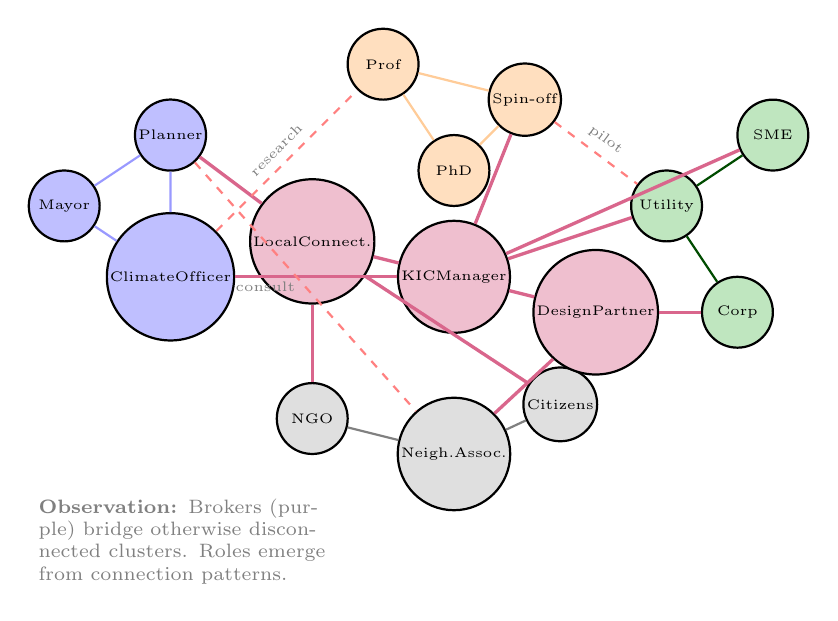
\begin{tikzpicture}[
    actor/.style={circle, draw, thick, fill=#1!25, minimum size=0.9cm, font=\tiny, inner sep=1pt},
    tie/.style={-, thick, #1},
    label/.style={font=\tiny, #1},
    scale=0.9
]
% Actors - positioned to show connection patterns
% City government cluster
\node[actor=blue] (planner) at (-4,2) {Planner};
\node[actor=blue] (climate) at (-4,0) {Climate\\Officer};
\node[actor=blue] (mayor) at (-5.5,1) {Mayor};

% University cluster
\node[actor=orange] (prof) at (-1,3) {Prof};
\node[actor=orange] (spinoff) at (1,2.5) {Spin-off};
\node[actor=orange] (phd) at (0,1.5) {PhD};

% Business cluster
\node[actor=green!60!black] (utility) at (3,1) {Utility};
\node[actor=green!60!black] (sme) at (4.5,2) {SME};
\node[actor=green!60!black] (corp) at (4,-0.5) {Corp};

% Citizens cluster
\node[actor=gray] (ngo) at (-2,-2) {NGO};
\node[actor=gray] (assoc) at (0,-2.5) {Neigh.\\Assoc.};
\node[actor=gray] (cit) at (1.5,-1.8) {Citizens};

% Intermediaries (emergent brokers)
\node[actor=purple] (kic) at (0,0) {KIC\\Manager};
\node[actor=purple] (connector) at (-2,0.5) {Local\\Connect.};
\node[actor=purple] (design) at (2,-0.5) {Design\\Partner};

% Intra-cluster ties (thin, same color)
\draw[tie=blue!40] (planner) -- (climate) -- (mayor) -- (planner);
\draw[tie=orange!40] (prof) -- (spinoff) -- (phd) -- (prof);
\draw[tie=green!30!black] (utility) -- (sme);
\draw[tie=green!30!black] (utility) -- (corp);
\draw[tie=gray] (ngo) -- (assoc) -- (cit);

% Cross-cluster ties via brokers (thick, purple)
\draw[tie=purple!60, very thick] (kic) -- (climate);
\draw[tie=purple!60, very thick] (kic) -- (spinoff);
\draw[tie=purple!60, very thick] (kic) -- (utility);
\draw[tie=purple!60, very thick] (kic) -- (sme);

\draw[tie=purple!60, very thick] (connector) -- (planner);
\draw[tie=purple!60, very thick] (connector) -- (ngo);
\draw[tie=purple!60, very thick] (connector) -- (cit);
\draw[tie=purple!60, very thick] (connector) -- (kic);

\draw[tie=purple!60, very thick] (design) -- (assoc);
\draw[tie=purple!60, very thick] (design) -- (corp);
\draw[tie=purple!60, very thick] (design) -- (kic);

% Direct cross-cluster ties (dashed, emerging)
\draw[tie=red!50, dashed] (spinoff) -- (utility) node[midway, above, label=gray, sloped] {pilot};
\draw[tie=red!50, dashed] (climate) -- (prof) node[midway, above, label=gray, sloped] {research};
\draw[tie=red!50, dashed] (planner) -- (assoc) node[midway, left, label=gray] {consult};

% Annotation
\node[anchor=north west, font=\scriptsize, text width=4cm, gray] at (-6,-3) {
    \textbf{Observation:} Brokers (purple) bridge otherwise disconnected clusters. Roles emerge from connection patterns.
};
\end{tikzpicture}
\caption{Ground-level actor connections in a Deep Demonstration site. Cluster structure and brokerage positions visible before role labels assigned.}
\label{fig:local-ties}
\end{figure}

%═══════════════════════════════════════════════════════════════════════════════
\section{Chapter Summary}
\labsec{role-constellations-summary}
%═══════════════════════════════════════════════════════════════════════════════

\begin{summarybox}
This chapter developed the theoretical framework for \textbf{role constellations}---relational configurations among actor roles that shape sustainability transition dynamics.

\textbf{Key theoretical elements:}
\begin{itemize}[leftmargin=*, itemsep=0.3em]
\item \textbf{Role constellations} are patterns of cooperation, competition, and mutual influence among actors occupying distinct transition roles

\item The \textbf{Multi-Actor Perspective} provides the institutional mapping (state, market, third sector, community) with intermediaries in hybrid positions

\item \textbf{Constellation dynamics} evolve across transition phases, from emergence through stabilization

\item \textbf{Research gaps} include weak theorization, static analysis, cross-level integration, and geographic/sectoral bias

\item The \textbf{eight EIT KICs} serve as probes into different sustainability domains, enabling comparative constellation analysis

\item \textbf{Roles emerge from connections}---structural position in networks determines functional role, not formal designation
\end{itemize}

The next chapters apply this framework empirically, mapping role constellations across the EIT ecosystem using multimodal cartography.
\end{summarybox}

\end{document}
